\subsection{Code structure}

The code\footnote{Code available on GitHub: \url{https://github.com/hws1302/partIII-project/tree/main/cartesian_mace}} was built using the \texttt{pytorch} package in python which allows for the  building and training of deep learning modules/architectures. I initially looked at using the \texttt{torch\_geometric.nn.MessagePassing} class which has message passing functionality built-in but eventually decided to build a bespoke architecture using instances of the ubiquitous \texttt{torch.nn.Module} class. \texttt{torch\_geometric} was used to store graph structured data in the \texttt{Data} class.  

\begin{figure}[H]
    \centering
    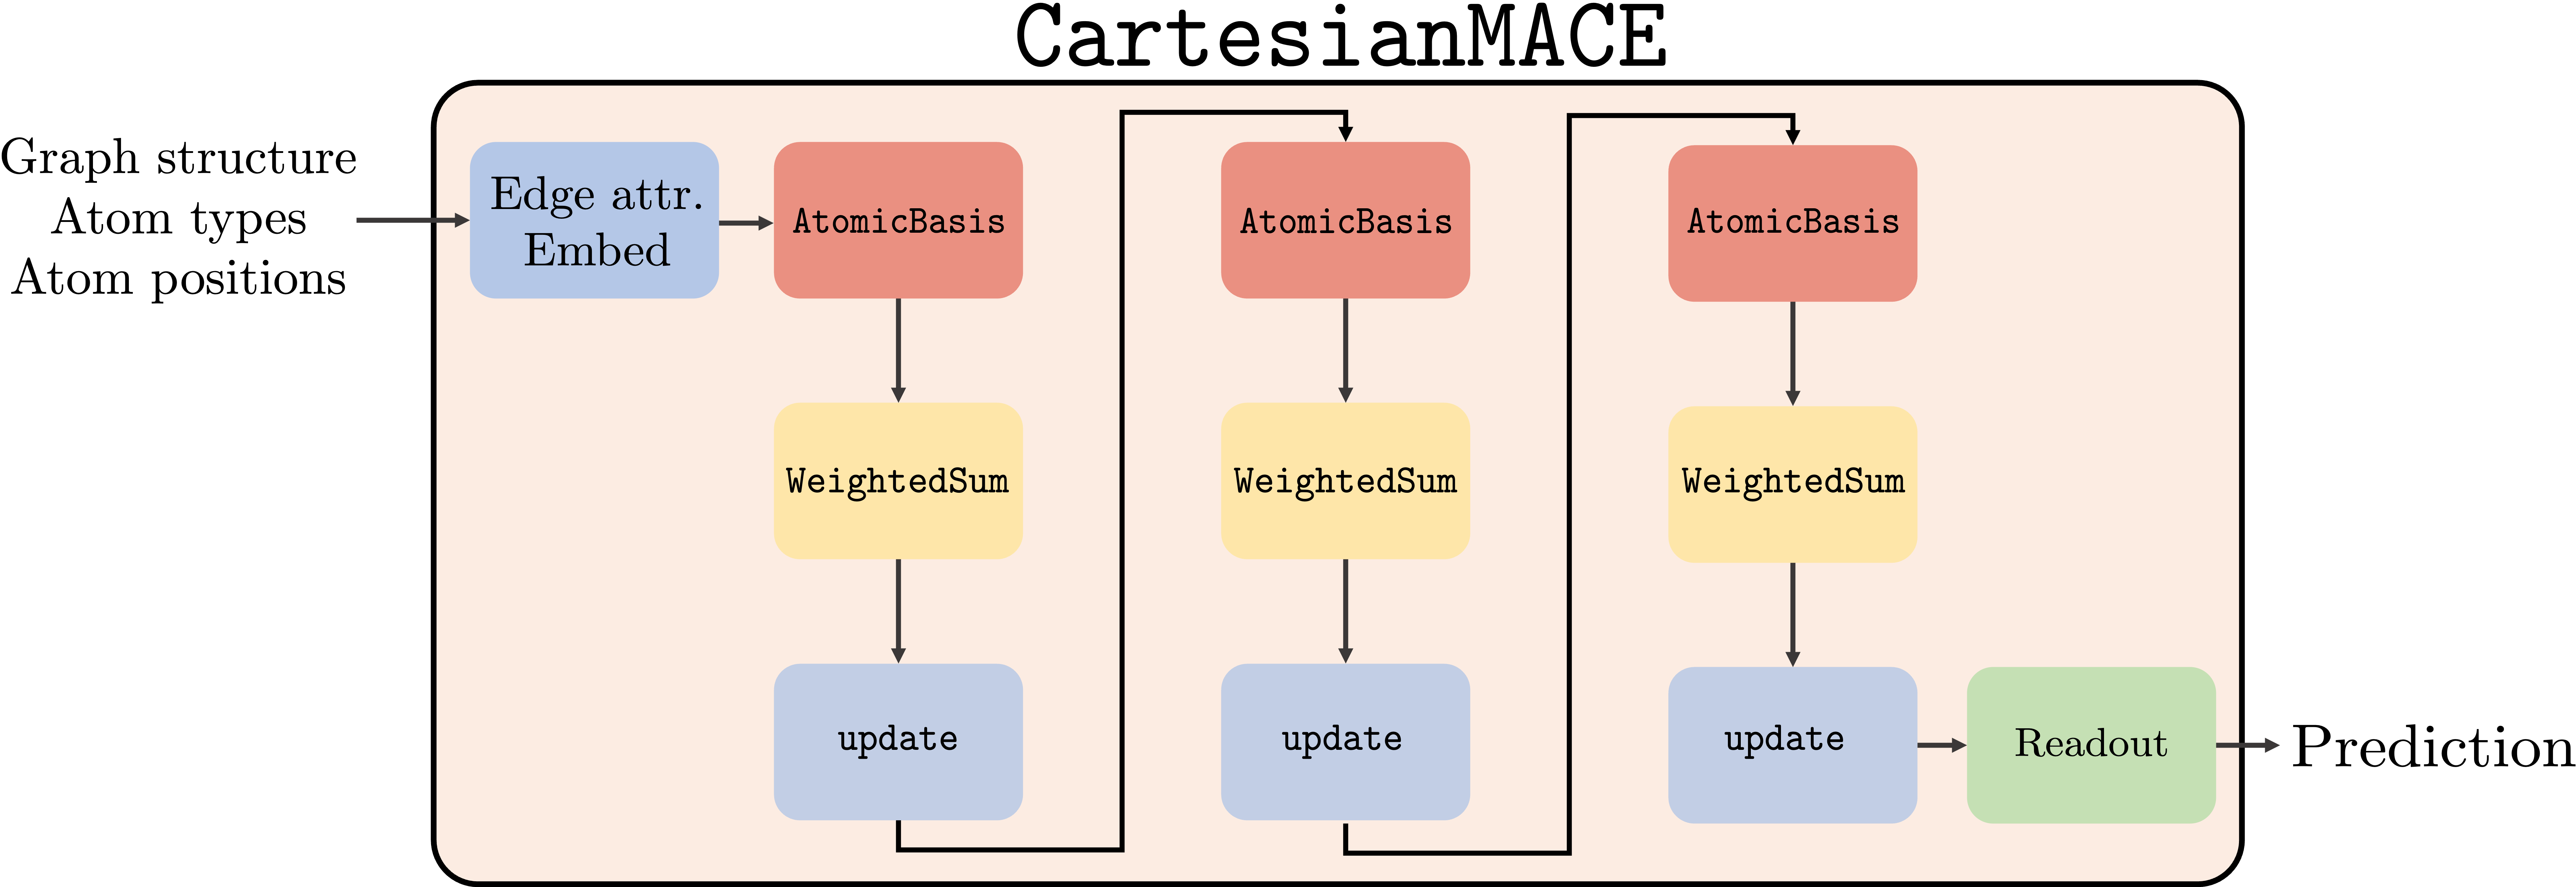
\includegraphics[width=0.8\textwidth]{figures/architecture.png}
    \caption{A CMACE model with 3 layers. To find initial features, embeddings are found using the atom type. Each layer is made from three modules: \texttt{AtomicBasis}, \texttt{WeightedSum} and \texttt{update} and outputs an updated set of features which can be the input for the next layer. After all the layers we use a readout function to get scalar output of model.}
    \label{fig:architecture}
\end{figure}


The model was assembled using three main classes. The \texttt{CartesianContraction} class carries out the exact same function as the Contraction operator (see Figure \ref{fig:contraction-op}) and abstracts away all of nuance of contractions so that the code for the other classes is much more readable. The \texttt{AtomicBasis} class completes the operations of Equations \ref{eq:phi} and \ref{eq:atomic-basis} by taking in the features and edge attributes derived off relative positions, produces the particle basis states which are summed to yield the atomic basis. The \texttt{WeightedSum} class carries out Equations \ref{eq:product}, \ref{eq:prod-con} and \ref{eq:message} by taking in the set of atomic basis tensors for each node, calculates all the splits and their contractions, then creates a linear sum of all the paths to a certain rank, hereby forming the message as in Figure \ref{fig:create-message}. The updating of Equation \ref{eq:update} takes place as a class method. These three parts are repeated in that order once per layer as seen in \ref{fig:architecture} which represents an instance of three layers. The final scalar feature are used as input to a readout function which in the case of our experiment was a \texttt{torch.nn.Linear} layer. 

\subsection{Optimisation}

\begin{figure}[H]
    \centering
    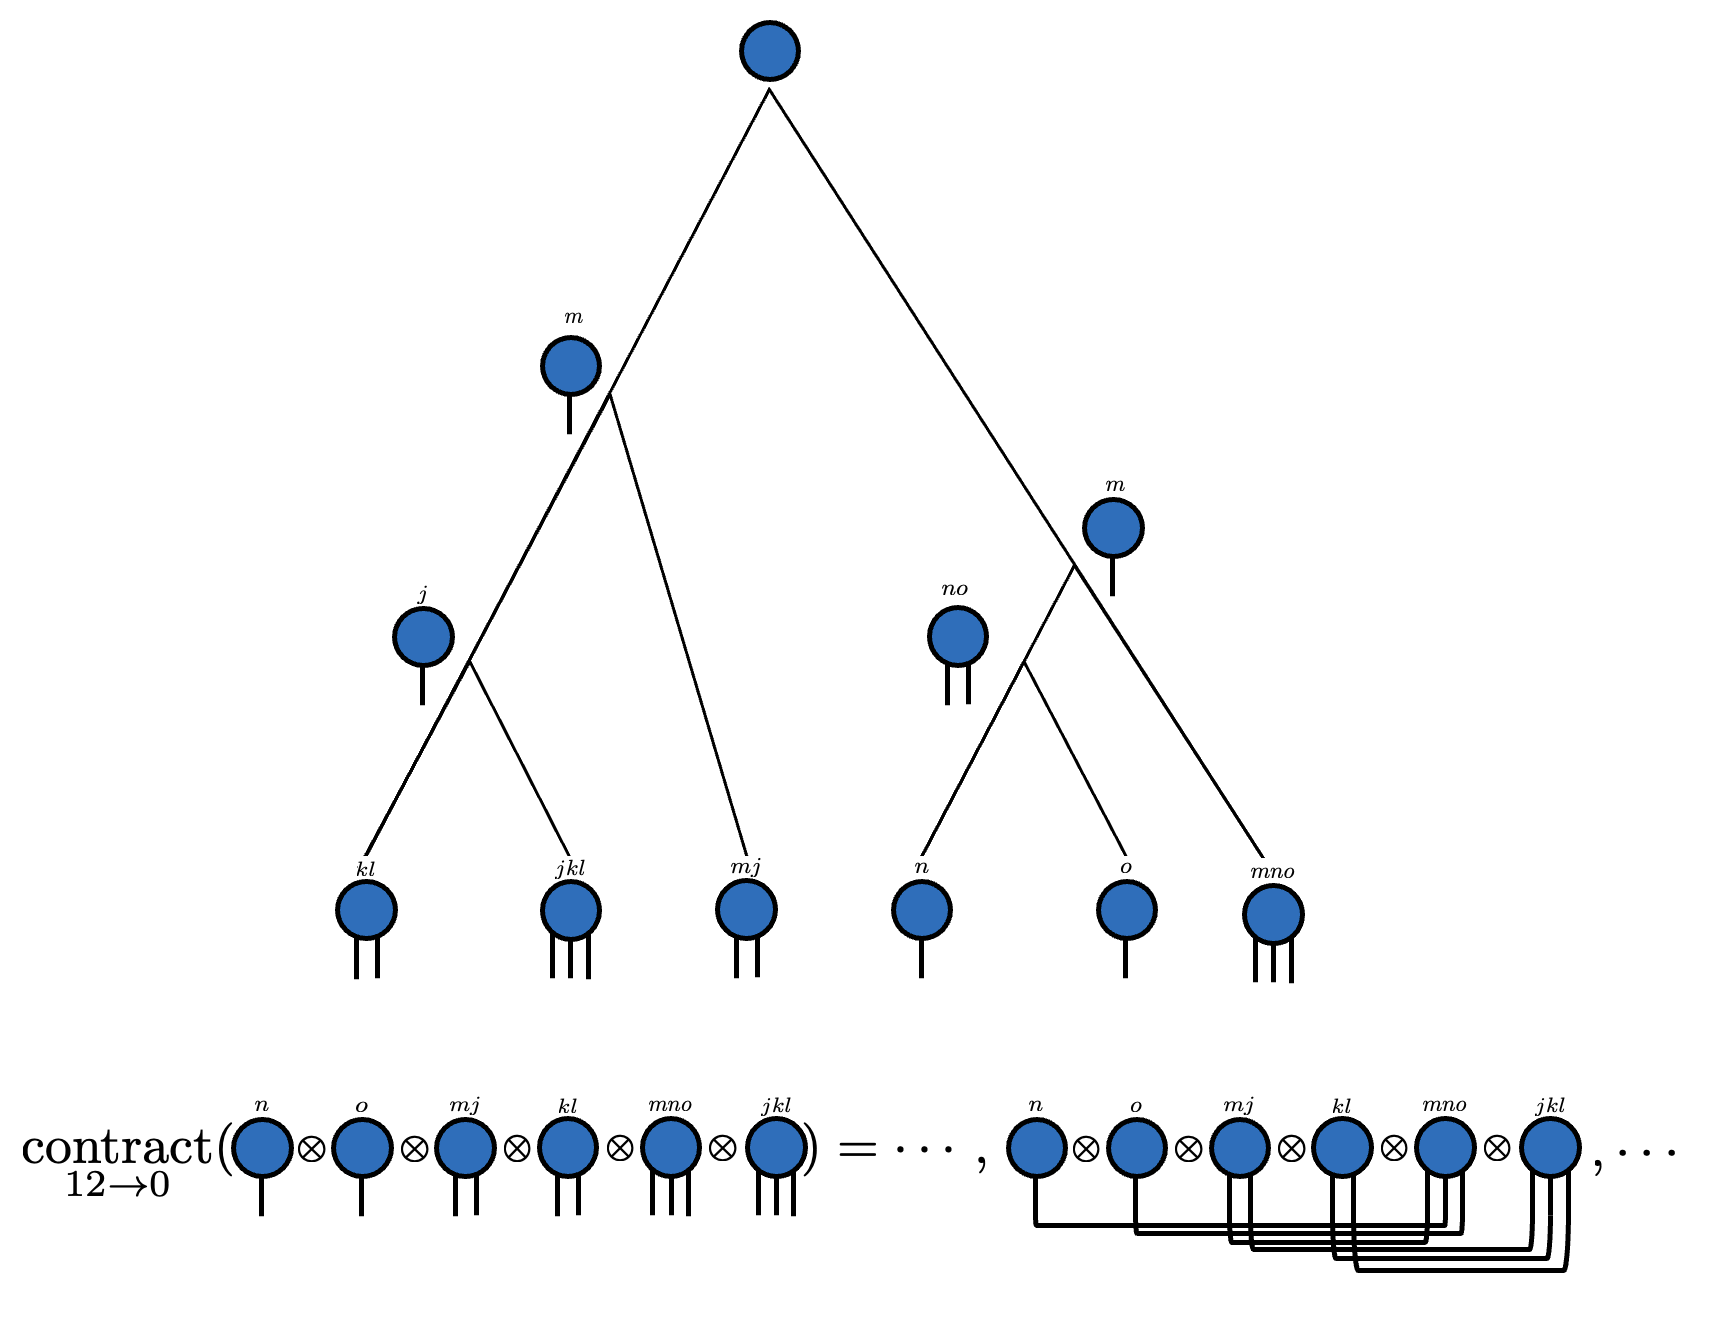
\includegraphics[scale=0.4]{figures/con-tree.png}
    \caption{bottom: one contraction combination of a tensor product of rank-12 to a scalar. top: the optimal order to contract in, this optimises both compute and memory requirements.}
    \label{fig:con-tree}
\end{figure}

The order in which the indices of a tensor are contracted doesn't affect the output values but makes a large difference to the computational cost. CMACE uses the \texttt{opt\_einsum} package to calculate near-optimal contraction paths, like the one seen in Figure \ref{fig:con-tree}. As finding paths is also computationally non-trivial the path saving feature of \texttt{opt\_einsum} is used. Table \ref{tab:con} shows that saving paths $>5 \times$ quicker vs. built-in PyTorch solution (find path at runtime). For a full discussion see Appendix \ref{sec:paths}.

\begin{table}[H]
    \centering
    \resizebox{0.9\textwidth}{!}{
    \begin{tabular}[width=0.6\textwidth]{lcccc}
    \toprule
    
        \textbf{Contraction method} & \textbf{Time /ms} & \textbf{Speed-up vs. na\"ive} &  &  \\
        \midrule
        Theoretical                 & -             & $31.0$                  &  & \\
        Saved path (\texttt{opt\_einsum})                  & $0.34 \pm     0.02$       & $26.7$                   &  &  \\
        Find path at runtime (\texttt{opt\_einsum})               & $1.79 \pm 0.03$            & $5.3$                   &  &  \\
        Naive path (\texttt{numpy})         & $9.52 \pm 0.12$             & $1.0$                  &  & 
     \\ \toprule
    \end{tabular}
    }
    \caption{The runtimes of different tensor contraction methods compared to the theoretical speed up of optimal path by \texttt{opt\_einsum}. This shows us that \textbf{saving paths is >5 \times quicker than calculating at runtime}
    }
    \label{tab:con}
\end{table}


